\documentclass[a4paper]{article}

%% Language and font encodings
\usepackage[portuges]{babel}
%\usepackage{fontspec}

%% Sets page size and margins
\usepackage[a4paper,top=3cm,bottom=2cm,left=3cm,right=3cm,marginparwidth=1.75cm]{geometry}

%% Useful packages
\usepackage{amsmath,amsthm,amssymb,amsfonts}
\usepackage{graphicx}
\usepackage[colorinlistoftodos]{todonotes}
\usepackage[colorlinks=true, allcolors=blue]{hyperref}
\usepackage{subfig}
\usepackage{float}



\newcommand{\R}{\mathbb{R}}
\newcommand{\N}{\mathbb{N}}
\newcommand{\Z}{\mathbb{Z}}
\providecommand{\C}{\mathbb{C}}

\theoremstyle{definition}
\newtheorem{defin}{Definição}

\theoremstyle{plain}
\newtheorem{theorem}[defin]{Teorema}
\newtheorem{corollary}[defin]{Corolário}



\title{Laboratório de CEME - Lab 2\\Simulação de um sistema eletromecânico: Contatora}

\author{Cleiton M. Freitas\\
}

\date{}

\begin{document}
\maketitle

%\begin{abstract}
%Your abstract.
%\end{abstract}

%%%%%%%%%%%%%%%%%%%%%%%%%%%%%%%%%%%%%%%%%%
%%%%%%%%%%%%%%%%%%%%%%%%%%%%%%%%%%%%%%%%%%
%%%%%%%%%%%%%%%%%%%%%%%%%%%%%%%%%%%%%%%%%%
\section{Objetivo}

O objetivo desta experiência é montar a simulação de um sistema eletromecânico simples, o sistema de uma contatora. 

%%%%%%%%%%%%%%%%%%%%%%%%%%%%%%%%%%%%%%%%%%
%%%%%%%%%%%%%%%%%%%%%%%%%%%%%%%%%%%%%%%%%%
%%%%%%%%%%%%%%%%%%%%%%%%%%%%%%%%%%%%%%%%%%
\section{A contatora}


Uma contatora é um sistema geralmente utilizado como chave eletromecânica.


\begin{figure}
\centering
\subfloat[$i = 0$]{
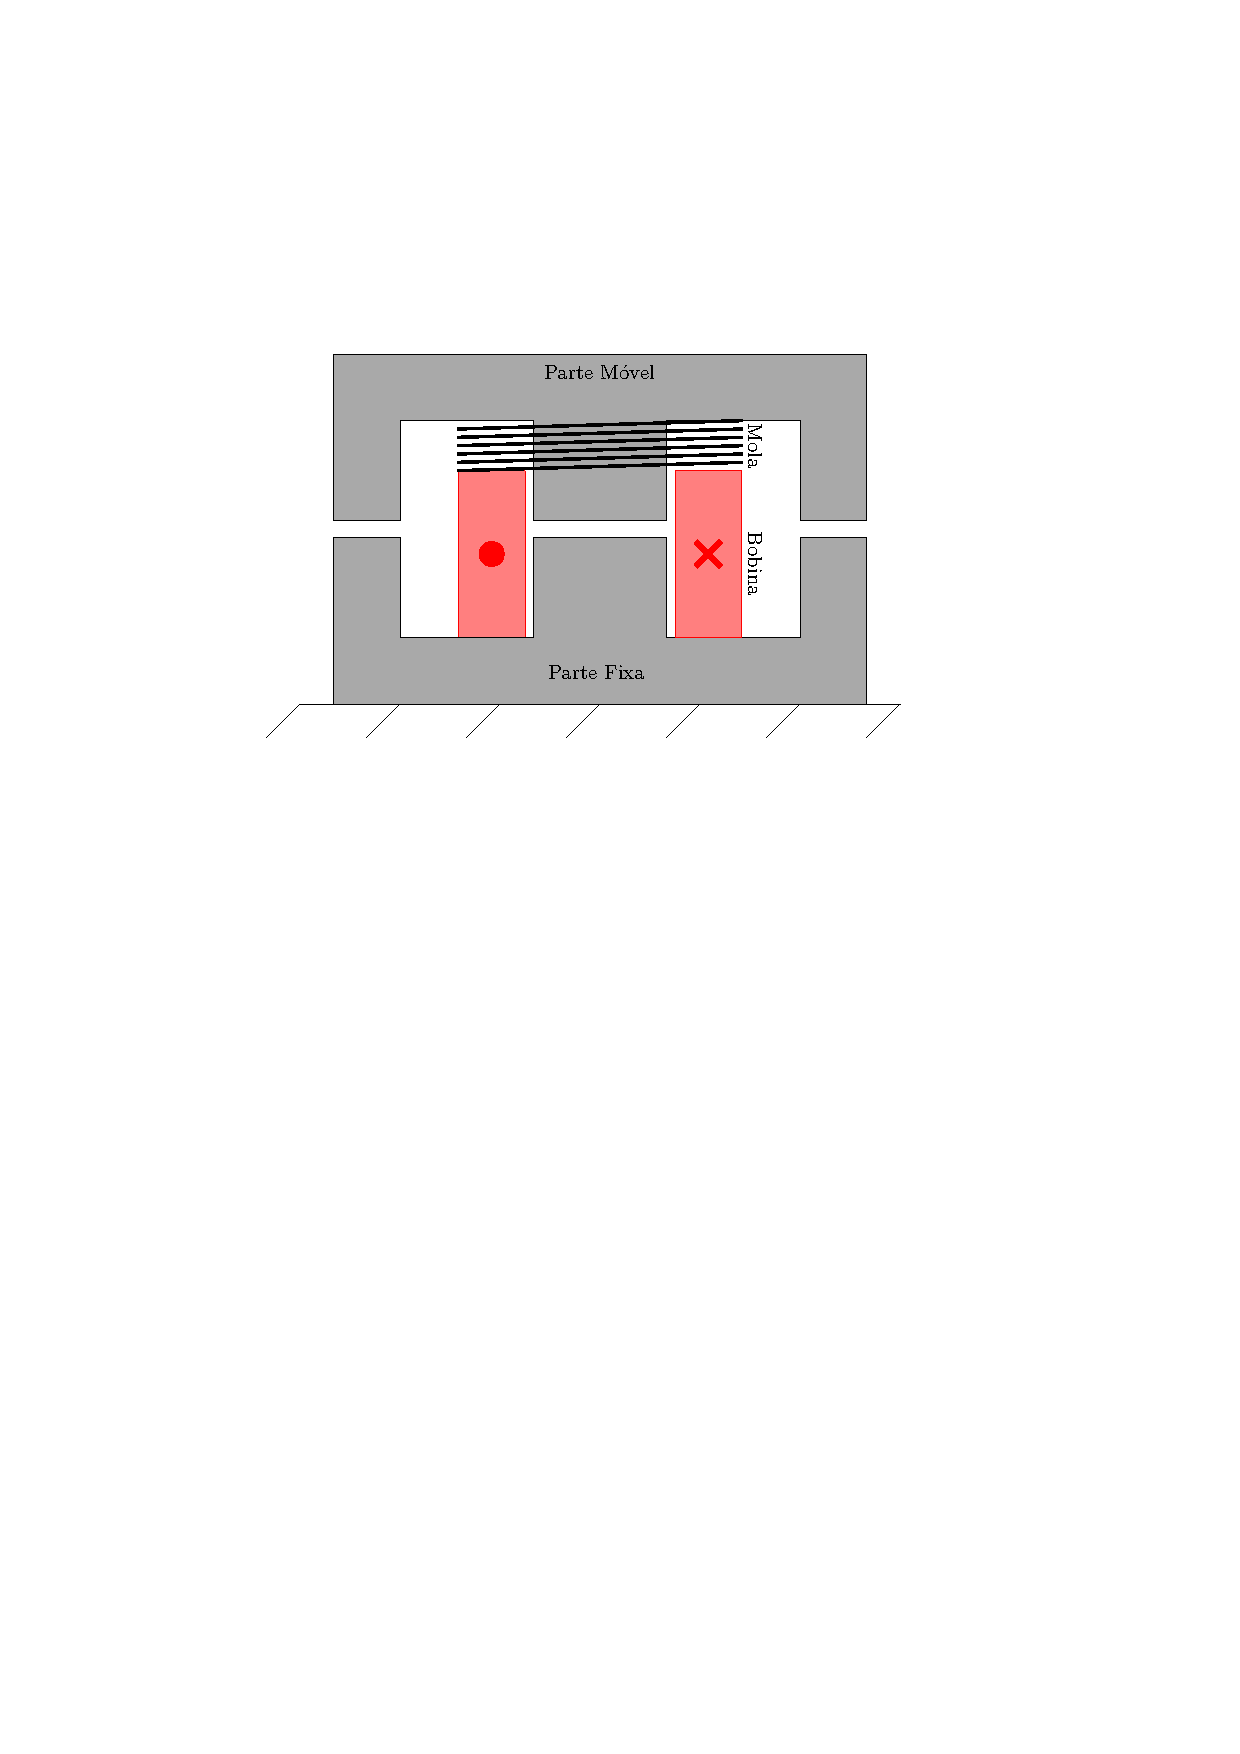
\includegraphics[width=0.48\linewidth]{./figuras/contatora_0}
}
\subfloat[$i \neq 0$]{
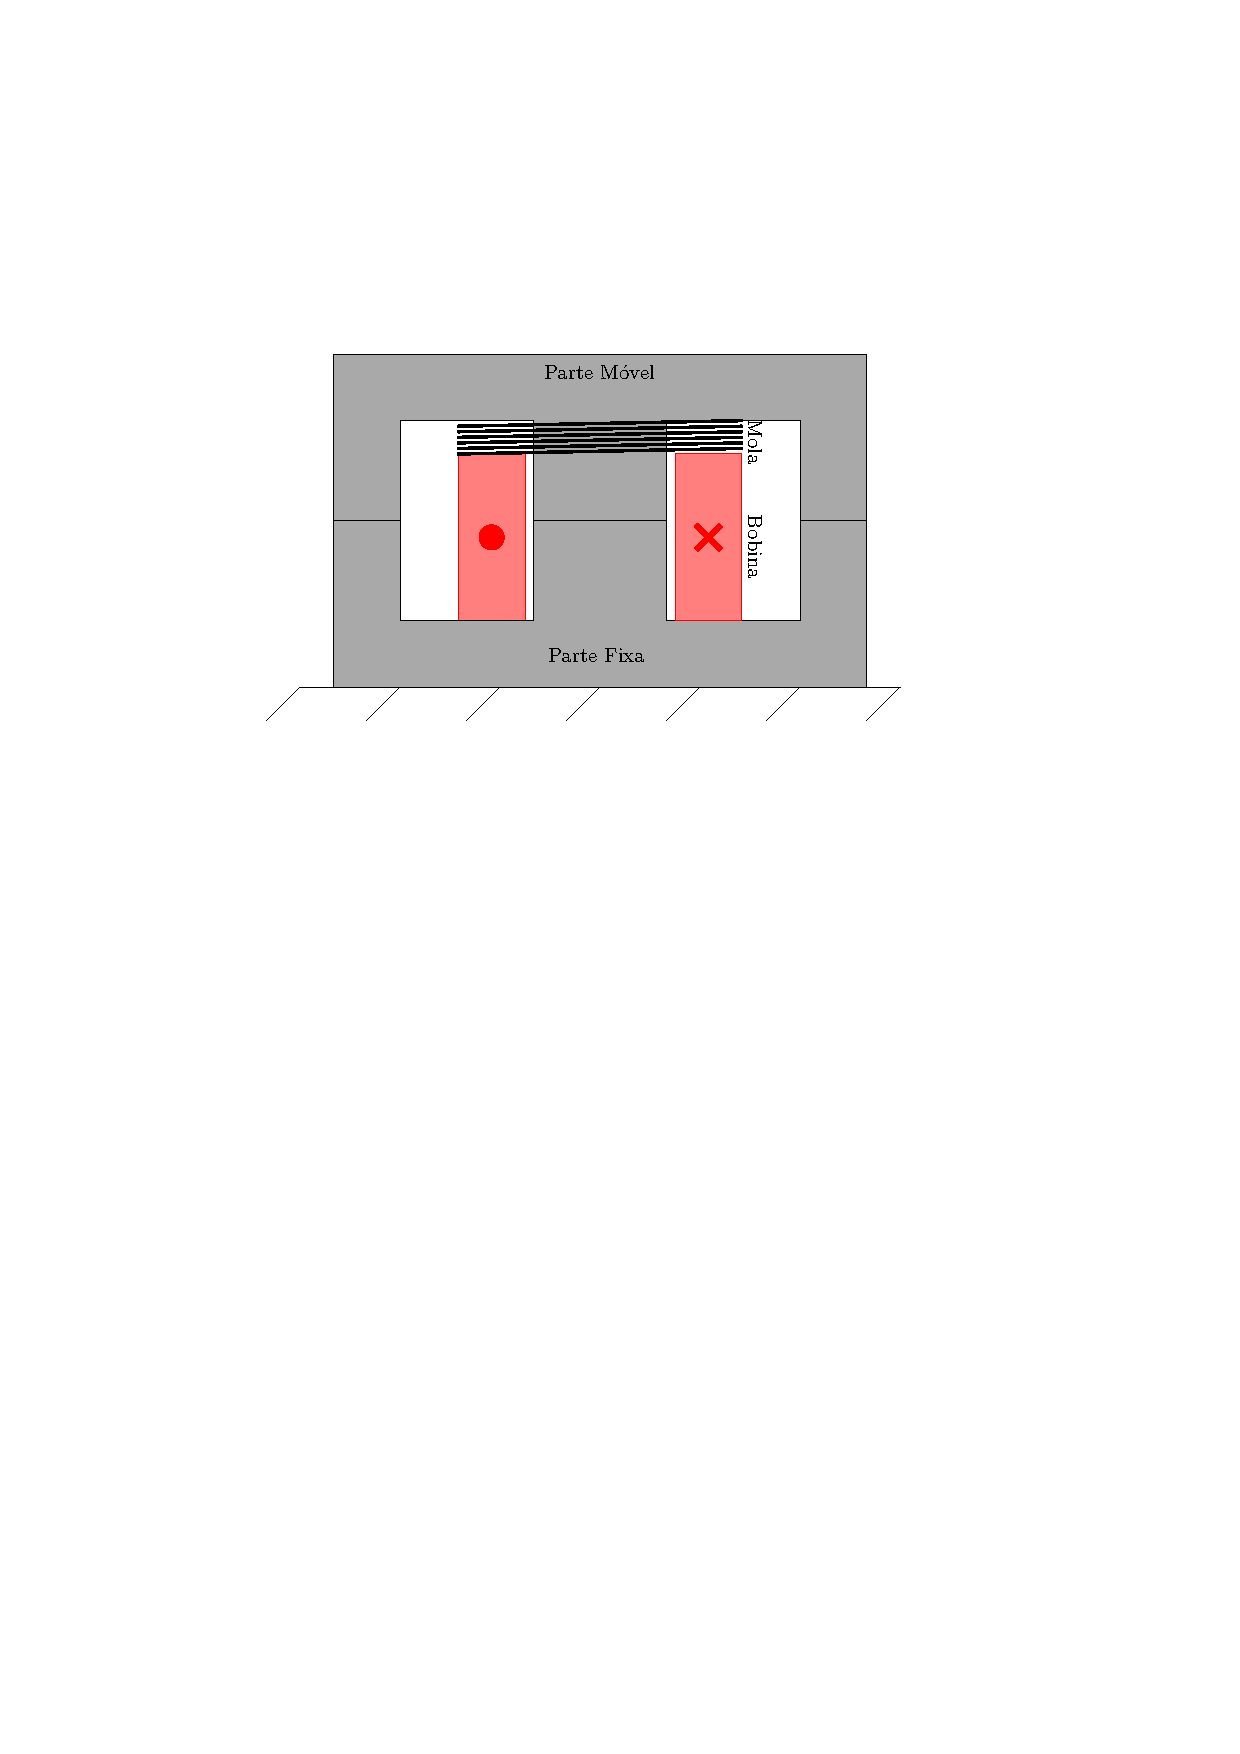
\includegraphics[width=0.48\linewidth]{./figuras/contatora_1}
}
\caption{Esquema de uma contatora}
\end{figure}

 
 %https://www.youtube.com/watch?v=JHKL6CwKntQ&t=181s
 %https://www.youtube.com/watch?v=OKiCSIbYXBU


%%%%%%%%%%%%%%%%%%%%%%%%%%%%%%%%%%%%%%%%%%
%%%%%%%%%%%%%%%%%%%%%%%%%%%%%%%%%%%%%%%%%%
%%%%%%%%%%%%%%%%%%%%%%%%%%%%%%%%%%%%%%%%%%
\section{Desenvolvimento das Simulações do transformador}


A Figura~\ref{fig:trafo:quadri} possui a representação em quadripolo\footnotemark de um transformador monofásicos. Neste circuito, $i_1$ e $i_2$ são as correntes que entram nos enrolamentos primário e secundário do transformador. Além disso, $e_1$ e $e_2$ são as tensões induzidas destes enrolamentos. A caixa nomeada \textbf{Sistema Eletromag.}, por sua vez, representa a interação eletromagnética no circuito. Ou seja, ela representa as seguintes equações:

\begin{equation}
\begin{bmatrix}
\lambda_1(t)\\[5pt]
\lambda_2(t)
\end{bmatrix} =
\begin{bmatrix}
L_{11} & L_{12}\\[5pt]
L_{21} & L_{22}
\end{bmatrix}
\begin{bmatrix}
i_1(t)\\[5pt]
i_2(t)
\end{bmatrix}
\label{eq:lambda}
\end{equation} 


\begin{equation}
\begin{bmatrix}
e_1(t)\\[5pt]
e_2(t)
\end{bmatrix} =
\frac{d}{dt} 
\begin{bmatrix}
\lambda_1(t)\\[5pt]
\lambda_2(t)
\end{bmatrix}
\label{eq:e}
\end{equation}


\footnotetext{Deixo como curiosidade a página sobre \href{https://pt.wikipedia.org/wiki/Quadripolo}{quadripolos} na Wikipedia. Este assunto sempre aparece nos últimos capítulos dos livros de circuito, mas por questão tempo nem sempre é abordado em aula.}

\begin{figure}[H]
\centering
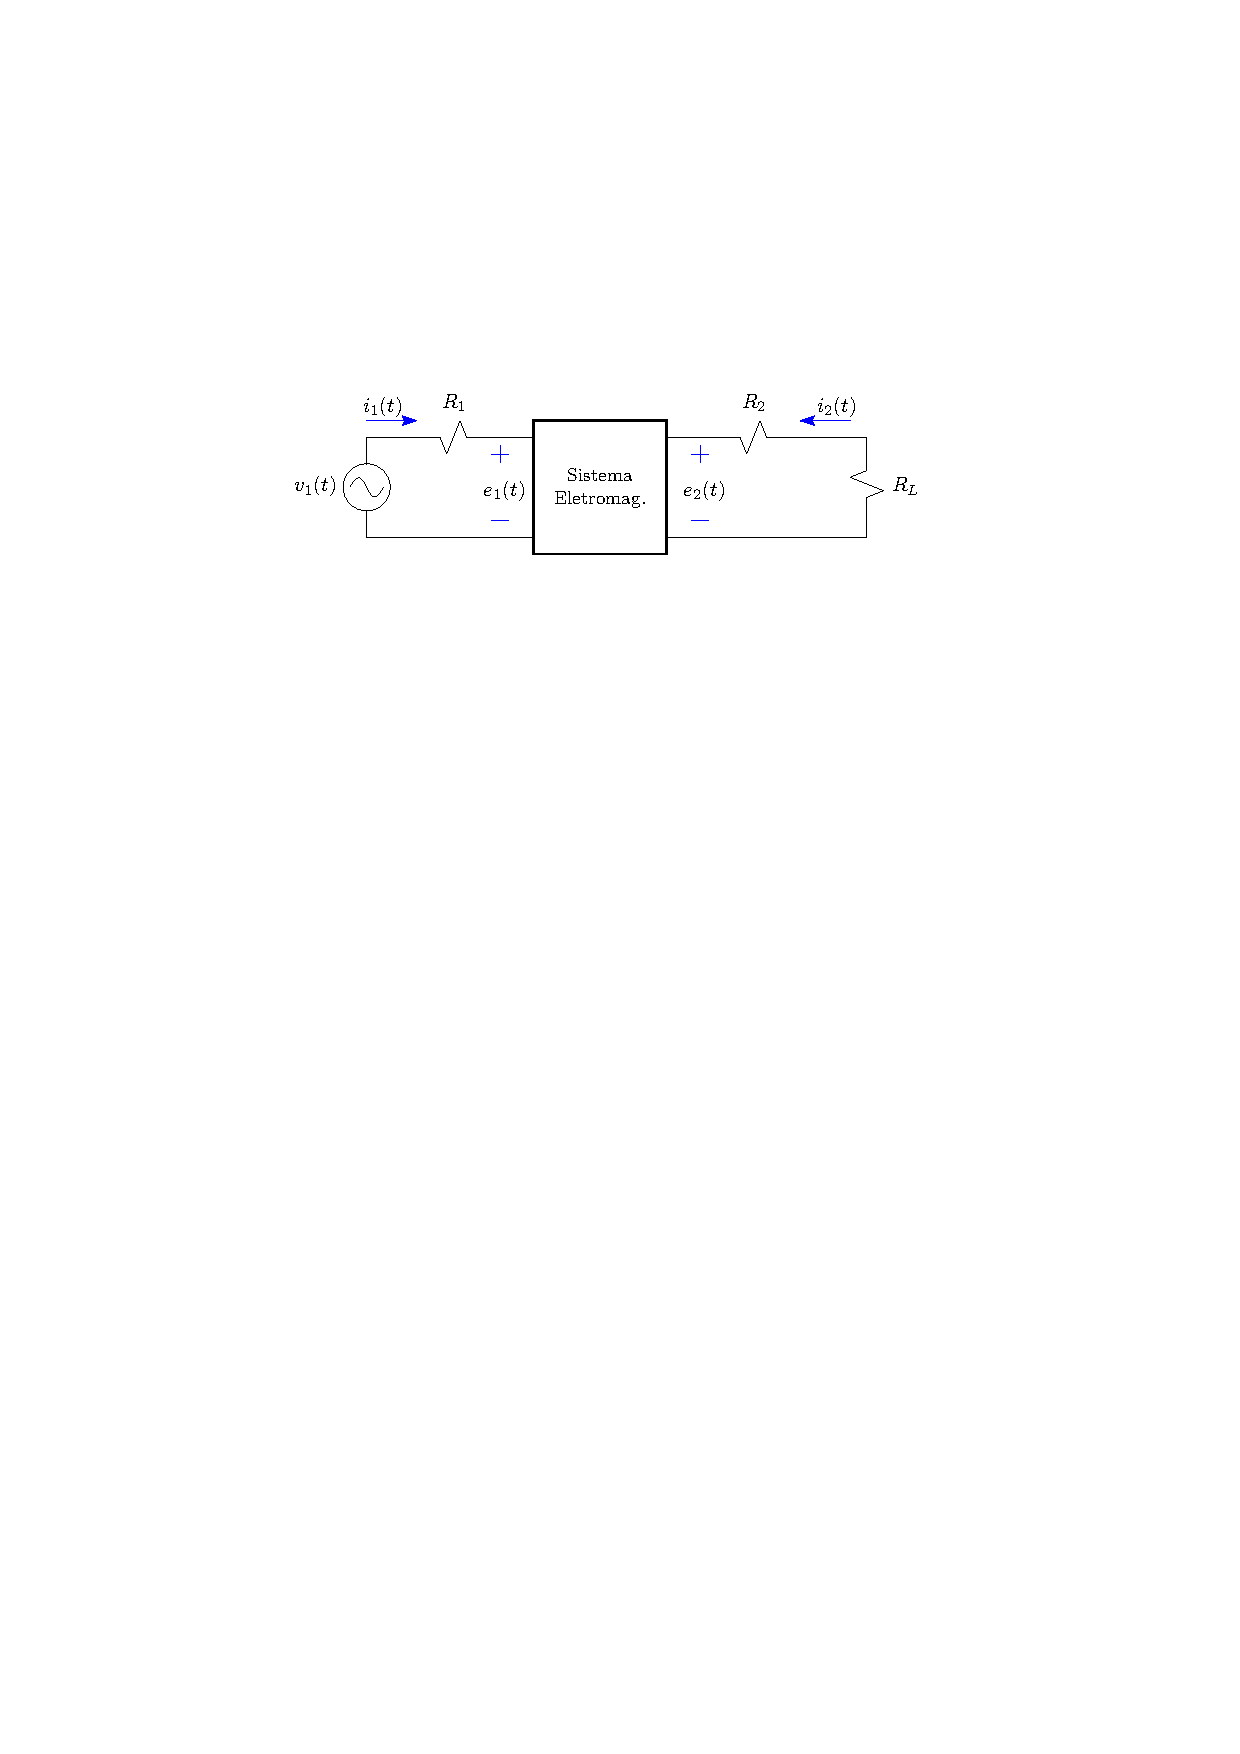
\includegraphics[width=0.75\linewidth]{../../Figuras/Trafo_mono_sistema_eletromag.pdf}
\caption{Representação em quadripolo do transformador}
\label{fig:trafo:quadri}
\end{figure}


O circuito ainda apresenta três resistências e uma fonte de tensão. $R_1$ e $R_2$ são as resistências dos enrolamentos e $R_L$ a resistência de carga.  

O primeiro objetivo da simulação é computar as correntes $i_1$ e $i_2$ neste circuito. Para isso, o primeiro passo é obter duas equações diferencias que descrevam estas correntes em função da tensão apicada no primário. Ou seja, obter o seguinte par de equações:

\begin{equation}
\frac{d i_1}{dt} = f_1(t,v_1, i_1, i_2)
\end{equation} 

\begin{equation}
\frac{d i_2}{dt} = f_2(t,v_1,  i_1, i_2)
\end{equation} 

Observe que as funções $f_1$ e $f_2$ são obtidas combinado a lei das malhas no circuito da figura~\ref{fig:trafo:quadri} com as equações (\ref{eq:lambda}) e (\ref{eq:e}). Quando montar as equações, utilize os sentidos de tensões e correntes indicados na figura, ou problemas numéricos poderão aparecer.


O segundo passo consiste em resolver este sistema de equações. Mas ao invés de seguir as metodologias aprendidas em Cálculo III, resolveremos este sistema de forma numérica usando \textbf{SciPy}. Mais especificamente, utilizando a função \verb|scipy.integrate.odeint|, que realiza a integração numérica de um sistema de equações diferencias de primeira ordem. O link a seguir possui um exemplo de utilização desta função para resolver um sistema de duas equações diferencias:

\begin{itemize}
\item \href{https://docs.scipy.org/doc/scipy/reference/generated/scipy.integrate.odeint.html}{scipy.integrate.odeint}
\end{itemize}

Após calcular as correntes com a função a função \verb|scipy.integrate.odeint|, podemos calcular fluxo concatenado e tensões induzidas utilizando as definições já apresentadas.




%%%%%%%%%%%%%%%%%%%%%%%%%%%%%%%%%%%%%%%%%%
%%%%%%%%%%%%%%%%%%%%%%%%%%%%%%%%%%%%%%%%%%
%%%%%%%%%%%%%%%%%%%%%%%%%%%%%%%%%%%%%%%%%%
\section{Dados do transformador}


Antes de apresentar os dados, é necessário definir alguns parâmetros que só serão apresentados no futuro nas aulas de teoria. Estes parâmetros são as indutâncias de magnetização ($L_{m1}$ e $L_{m2}$) e de dispersão ($L_{l1}$ e $L_{l2}$). A indutância de magnetização, como o nome já diz, representa a magnetização do transformador, ou seja, permite o calculo do fluxo que flui através das duas bobinas. As indutâncias de dispersão representam, por outro lado, se relacionam com as parcelas de fluxo que se espalha pelo ar.


\begin{table}[H]
\centering
\caption{Parâmetros do Transformador}
\begin{tabular}{ccc}
\hline
\textbf{Parâmetro} & \textbf{Notação} & \textbf{Valor}\\ \hline
Tensão nominal do primário & $V_1$ & 127V\\
Tensão nominal do secundário & $V_2$ & 480V\\
Potência nominal & - & 5kVA\\
Indutância de dispersão do primário & $L_{l1}$ & 0.42mH\\
Indutância de dispersão do secundário & $L_{l2}$ & 6.11mH\\ 
Indutância de Magnetização vista do primário & $L_{m1}$ & 0.17113H\\ 
Indutância de Magnetização vista do secundário & $L_{m2}$ & 2.44456H\\ 
Resistência da bobina primária & $R_{1}$ & 0.2$\Omega$\\ 
Resistência da bobina secundária & $R_{2}$ & 2.8$\Omega$\\ 
\hline
\end{tabular}
\end{table}

Pra fins de simplicidade, considere que os números de espiras $N_1$ e $N_2$ são numericamente iguais as tensões nominais.

De acordo com a referência \cite[Capítulo 1]{krause2013analysis}, as indutâncias próprias e mútuas de um transformador são dadas por:

\begin{equation}
\mathbf{L} = 
\begin{bmatrix}L_{11} & L_{12}\\[5pt] 
L_{21} & L_{22}\end{bmatrix} = 
\begin{bmatrix}L_{l1}+L_{m1} & \frac{N2}{N1} L_{m1}\\[5pt] 
\frac{N1}{N2} L_{m2} & L_{l2}+L_{m2}\end{bmatrix}
\end{equation}


É possível mostrar que:

\begin{equation}
\frac{N1}{N2} L_{m2} = \frac{N2}{N1} L_{m1}
\end{equation}


Utilize este resultados para obter as indutâncias próprias e mútuas do transformador.

%%%%%%%%%%%%%%%%%%%%%%%%%%%%%%%%%%%%%%%%%%
%%%%%%%%%%%%%%%%%%%%%%%%%%%%%%%%%%%%%%%%%%
%%%%%%%%%%%%%%%%%%%%%%%%%%%%%%%%%%%%%%%%%%
\section{Casos teste}

Uma vez que a simulação esteja funcionado, faça os casos testes apresentados a seguir. Em todos os casos, calcule e plote as correntes, os fluxos concatenados e as tensões induzidas. Além disso, para visualizar todos os efeitos, realize simulações com diferentes durações (de algumas dezenas de ms até alguns segundos).


\begin{enumerate}
\item \textbf{Caso 1:} Considere o transformador alimentado com tensão alternada nominal com 60Hz. Ou seja:

\begin{equation}
v_1(t) = \sqrt{2}V_1 \sin(\omega t)
\end{equation}

onde $\omega = 2 \pi 60 = 120\pi$. Considere também que a carga possui $47\Omega$.

\item \textbf{Caso 2:} Considere a mesma tensão do caso anterior, mas desta vez use uma carga de $10k\Omega$.


\item \textbf{Caso 2:} Considere a carga de $47\Omega$, mas no lugar de uma fonte alternada, alimente o transformador com uma fonte CC de $2V$ 

\end{enumerate}









\bibliographystyle{plain}
\bibliography{referencias}




\end{document}